\documentclass[conference]{IEEEtran}
\usepackage{cite}
\ifCLASSINFOpdf
  \usepackage[pdftex]{graphicx}
  \graphicspath{{images/}}
\else
  \usepackage[dvips]{graphicx}
  \graphicspath{{images/}}
\fi
\usepackage[cmex10]{amsmath}
\interdisplaylinepenalty=2500
\usepackage{algorithmic}
\usepackage{array}
\ifCLASSOPTIONcompsoc
 \usepackage[caption=false,font=normalsize,labelfont=sf,textfont=sf]{subfig}
\else
 \usepackage[caption=false,font=footnotesize]{subfig}
\fi
\usepackage{fixltx2e}
%\usepackage{stfloats}
%\fnbelowfloat
% \usepackage{dblfloatfix}
\usepackage{url}

\hyphenation{op-tical net-works semi-conduc-tor}

\begin{document}

\title{GPU Accelerated Skeleton Tracking From a single Depth Image}

\author{\IEEEauthorblockN{
  Luke Fraser\IEEEauthorrefmark{1},
  Monica Nicolescu\IEEEauthorrefmark{2}, 
  Freddrick Harris\IEEEauthorrefmark{3},
  Lee Barford\IEEEauthorrefmark{4}}
}

\maketitle

\begin{abstract}
Skeleton tracking is an important component of robotics. Receiving high frequency and precise pose estimates from a person are useful when a robot interacts with a person. Knowing where a person allows for more accurate real-time planning. In this paper we present a skeleton tracking algorithm that provides accurate high resolution pose estimations in real-time. This is achieved through the use of the GPU as a GPGPU(General Purpose Graphics Processing Unit). With the GPU performing the majority of the computation the CPU can attend to other tasks.
\end{abstract}

\IEEEpeerreviewmaketitle

\section{Introduction}
\label{sec:intro}
Skeleton tracking is a very useful tool in many fields of computer science. Whether in human computer interaction, computer vision, robotics, graphics, and etc, skeleton tracking plays an important role in understanding human actions and behaviors. A lot of work has been done on the implementation of skeleton tracking \cite{Ganapathi2010,Bleiweiss2009,Baak2011,Plagemann2010,Knoop2009}. The methods can be broken down into several groups:(TODO: List groups). The most notable method is the data driven\cite{Baak2011,export:145347}(TODO: other data driven methods). It has had the most success and has produced the most robust trackers.

\subsection{Skeleton Tracking}
\label{subsec:skel}
Data driven methods have produced robust real-time solutions to skeleton tracking\cite{Baak2011}. These approaches either train a classifier or validate against a large dataset of poses.(TODO: Microsoft) produced a data driven method by training against a large set of a priori pose sets. The model was built from a very large data set of different people in different poses with a priori joint location information. Most data driven methods build a database of poses to compare against and then lookup the position of the current pose from the database at runtime. This allows the for low computation and quick convergence onto a solution for a given pose. However, data driven approaches rely on the a database that is complete. If the user moves into a pose that is not in the database then the system will fail.

In \cite{Baak2011} the authors were able to achieve 60 fps on the Swiss-Ranger 4000. 60 fps is a good rate for real-time robotics applications. This would provide the speed necessary for real-time robotic intent recognition. However, this speed was achieved at low resolutions where the number of pixels in the depth image are manageable. 

\subsection{Cuda GPU Model}
\label{subsec:cudaModel}
General Purpose programming on a Graphics processing unit (GPGPU) is a method of using the graphics pipeline of a GPU to massively parallelize standard algorithms. The graphics pipeline of a computer is inherently parallel and GPU is optimized to function for this purpose. Converting algorithms from the CPU model to the GPGPU is a non-trivial problem. The GPU model provides many challenges and limitations on the programmer. The GPU has far less memory than the CPU and as well it becomes very obvious early on that the performance of the GPU is very sensitive. It is important to manage operations carefully to make sure that the GPU's parallelism isn't lost. The GPU is very good at parallel task, but does not perform sequential operations well as is far slower than a CPU.

\begin{figure}[!t]
\centering
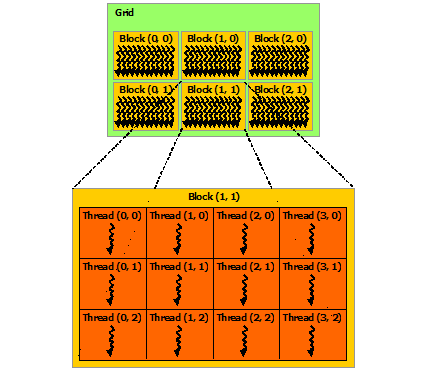
\includegraphics[width=2.5in]{grid-of-thread-blocks}
\caption{CUDA Thread model with grid and block structure containers.}
\label{fig:gridthreadblocks}
\end{figure}
\subsubsection{The CUDA Programming Model}
CUDA is defined by Nvidia\texttrademark, a GPU manufacturer\cite{Nvidia2014}. They have developed a general purpose programming model and language to implement programs on their GPU's. The programming model is described in detail in \cite{Nvidia2014}. A general outline of the CUDA model and programming paradigm will be outlined here.

The CUDA programming language is similar to C/C++ and much of the syntax is exactly the same. In fact the GCC compiler is called by the NVCC compiler to build a program. Central to programming for an Nvidia GPU is understanding how a CUDA kernel is executed. A host-machine executes the main program on the CPU and then makes kernel call request to the GPU which then runs the kernel on the GPU. Kernel calls are asynchronous operations and do not stall the CPU program from running. The host machine program can then perform memory transfers from the GPU to pass information back and forth between the CPU and GPU.

CUDA breaks down kernel function execution with 3 structuring elements, Grids, Blocks, and Threads. Threads are the element that executes a kernel function. Each thread executes the kernel function independently of the others. A thread has its own memory to store local variables. A block is a container for threads. A single block will have many threads that execute a given kernel function. Blocks as well have memory that all of their threads have access to. This memory is called shared memory and is only accessible to a blocks threads. A grid is a container for blocks. Unlike threads there is no shared memory between blocks of threads there is only global memory. This means that a thread of one block does not know anything about a thread of a different block. This is a critical issue that requires consideration when implementing an algorithm. Figure~\ref{fig:gridthreadblocks} shows the organization of threads, blocks, and grids.


\subsubsection{The CUDA Memory Hierarchy}
CUDA also employs a specific memory model on the kernel functions that execute on the GPU. Each thread has a small amount of local memory that it can use. As well each block has shared memory that all of its threads can access together. Grids all have access to the global memory of the GPU. The speed of the different types of memory is critical to the speed of a given algorithm on the GPU. Local memory is the fastest followed by block shared memory and then global memory. Figure~\ref{fig:memoryhierarchy} shows the accesses and structure of the GPU memory.

\begin{figure}[!t]
\centering
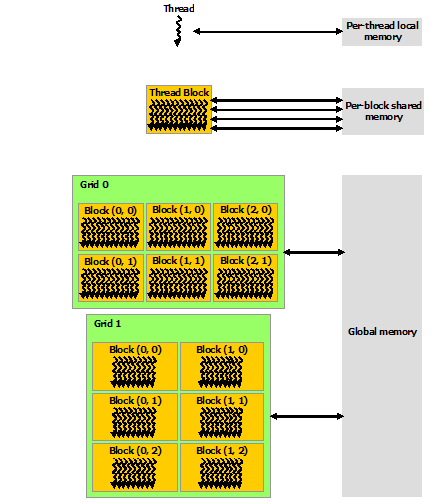
\includegraphics[width=2.5in]{memory-hierarchy}
\caption{CUDA memory hierarchy.}
\label{fig:memoryhierarchy}
\end{figure}

\section{Related Work}
\label{sec:relatedwork}

In the remaining sections a description of the methods developed for skeleton tracking will be discussed. As well a discussion of the results will be presented. The conclusion will list future work as well as the short comings of the project.
\section{Methods}
\label{sec:method}

\section{Conclusion}
\label{sec:clonclusion}


%\begin{figure}[!t]
%\centering
%\includegraphics[width=2.5in]{myfigure}
% where an .eps filename suffix will be assumed under latex, 
% and a .pdf suffix will be assumed for pdflatex; or what has been declared
% via \DeclareGraphicsExtensions.
%\caption{Simulation results for the network.}
%\label{fig_sim}
%\end{figure}

%\begin{figure*}[!t]
%\centering
%\subfloat[Case I]{\includegraphics[width=2.5in]{box}%
%\label{fig_first_case}}
%\hfil
%\subfloat[Case II]{\includegraphics[width=2.5in]{box}%
%\label{fig_second_case}}
%\caption{Simulation results for the network.}
%\label{fig_sim}
%\end{figure*}

%\begin{table}[!t]
%% increase table row spacing, adjust to taste
%\renewcommand{\arraystretch}{1.3}
% if using array.sty, it might be a good idea to tweak the value of
% \extrarowheight as needed to properly center the text within the cells
%\caption{An Example of a Table}
%\label{table_example}
%\centering
%% Some packages, such as MDW tools, offer better commands for making tables
%% than the plain LaTeX2e tabular which is used here.
%\begin{tabular}{|c||c|}
%\hline
%One & Two\\
%\hline
%Three & Four\\
%\hline
%\end{tabular}
%\end{table}


% \section*{Acknowledgment}

% trigger a \newpage just before the given reference
% number - used to balance the columns on the last page
% adjust value as needed - may need to be readjusted if
% the document is modified later
%\IEEEtriggeratref{8}
% The "triggered" command can be changed if desired:
%\IEEEtriggercmd{\enlargethispage{-5in}}

\bibliographystyle{IEEEtran}
% argument is your BibTeX string definitions and bibliography database(s)
\bibliography{IEEEabrv,refs/master}

\end{document}
